\documentclass[../diplomski_rad.tex]{subfiles}

\begin{document}

\sloppy

\justifying

Za učinkovitu primjenu ranije opisanog sustava potrebno je 
razviti ispitno okruženje koje omogućava ne samo prikupljanje podataka, 
već i njihovu analizu i interpretaciju na brz i intuitivan način.
U skladu s tim, u sklopu ovog rada razvijena je Python desktop aplikacija. 
Za izradu grafičkog sučelja korištena je biblioteka Qt i program Qt Designer pri čemu je 
naglasak stavljen na jednostavnost i intuitivnost korištenja.
Sve ikone korištene u aplikaciji besplatno su preuzete s Icons8 web stranice \cite{ikone}.

\begin{figure}[htb]
    \centering
    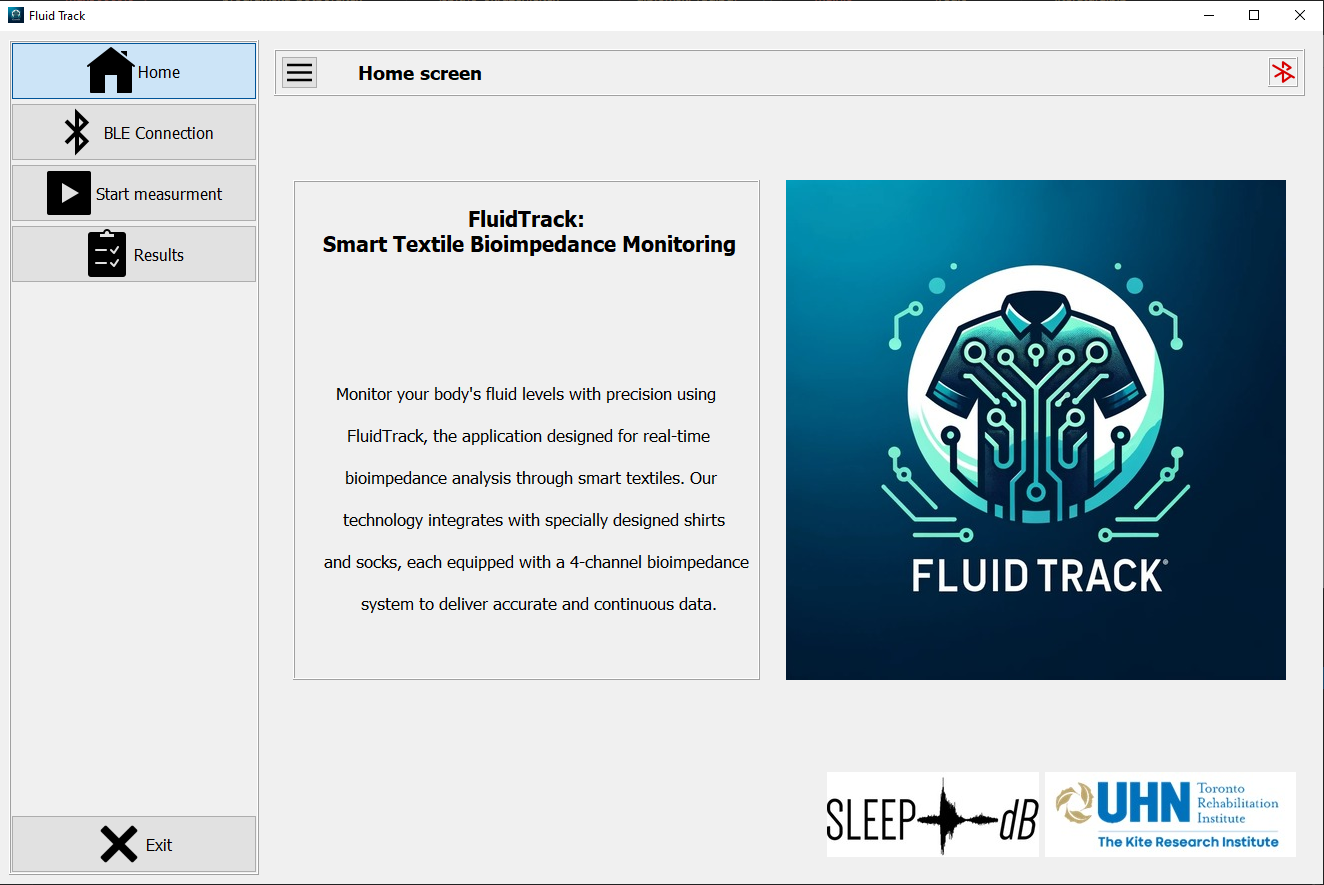
\includegraphics[width=0.85\textwidth]{Figures/home.png} 
    \caption{Početni zaslon razvijene aplikacije}
    \label{slk:home}
\end{figure}

Aplikacija omogućava povezivanje s razvijenim uređajem putem BLE komunikacijskog protokola, 
unos podataka o pacijentu,  
praćenje mjerenja u stvarnom vremenu te prikaz rezultata analize podataka. 
Podatci o pacijentima i mjerenja pohranjuju se u lokalnu bazu podataka. 
Pojedino mjerenje vezano je za pacijenta, čime se dobiva mogućnost praćenja pacijenata 
tijekom duljeg vremenskog razdoblja i usporedba različitih mjerenja za istog pacijenta.
Početni zaslon prikazan je na slici \ref{slk:home}. 
S lijeve strane ekrana tijekom cijelog rada aplikacije nalazi se izbornik kojim se korisnik lako prebacuje 
na željenu funkcionalnost.  

U nastavku će detaljno biti opisani implementacija i korištenje razvijenog ispitnog okruženja.

\section{Povezivanje s razvijenim uređajem}

Ispitno okruženje konfigurirano je kao BLE klijent te se jednostavno spaja na razvijeni nosivi uređaj. 
Pritiskom na karticu izbornika \texttt{BLE Connection} otvara se zaslon prikazan na slici \ref{slk:ble} 
koji korisniku pruža mogućnost upravljanja BLE konekcijom.

\begin{figure}[htb]
    \centering
    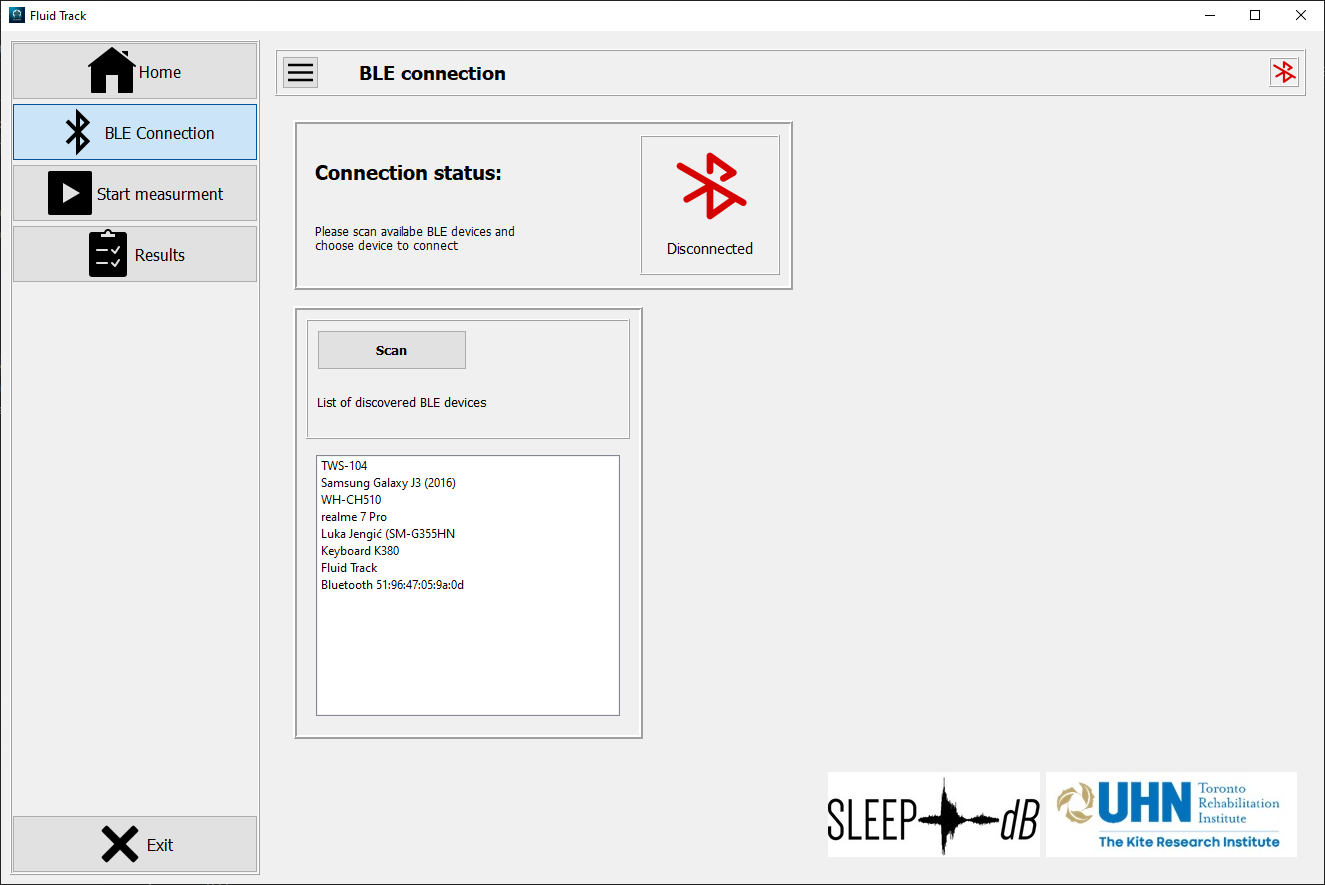
\includegraphics[width=0.85\textwidth]{Figures/ble.png} 
    \caption{Zaslon za upravljanje BLE vezom}
    \label{slk:ble}
\end{figure}

Status konekcije lako je vidljiv pomoću simbola BLE konekcije prikazanih na slici \ref{slk:ble_status_simboli}.  
Ako je simbol zelen, razvijeni sustav povezan je s ispitnim okruženjem dok u slučaju crvenog simbola konekcija nije uspostavljena.

\begin{figure}[htb]
    \centering
    
\includegraphics[width=0.4\textwidth]{Figures/ble_status_simboli.png} 
    \caption{Simboli oznake statusa BLE konekcije \cite{ikone}}
    \label{slk:ble_status_simboli}
\end{figure}

Pritiskom na tipku \texttt{Scan}  ispitno okruženje započinje skeniranje dostupnih uređaja 
u blizini putem BLE protokola. 
Nakon što se skeniranje završi, korisniku se prikazuje popis dostupnih uređaja na sučelju aplikacije.

Korisnik zatim ima mogućnost odabira željenog uređaja. Nakon što je uređaj odabran, pritiskom na tipku \texttt{Connect} 
pokreće se postupak povezivanja uređaja. 
Aplikacija obavještava korisnika o rezultatu pokušaja povezivanja te ako su uređaji uspješno povezani moguće je pokrenuti mjerenje.  
Za vrijeme dok su uređaji povezani na \texttt{BLE Connection} zaslonu prikazane su informacije o povezanom uređaju 
i tipka \texttt{Disconnect} kojom se korisniku daje mogućnost prekida BLE konekcije.

Za pokretanje mjerenja i prikupljanje mjernih podataka nužno je da aplikacija bude povezana s razvijenim nosivim sustavom. 
Zbog toga se prije početka mjerenja obavlja provjera je li aplikacija ostvarila BLE konekciju s razvijenim sustavom. 
Ako BLE konekcija nije ostvarena, aplikacija ne dozvoljava pokretanje mjerenja te korisnika o tome obavještava 
skočnim prozorom prikazanim na slici \ref{slk:ble_not_connected}. Tipka \texttt{Connect} na skočnom prozoru korisnika 
vodi na karticu \texttt{BLE Connection}.

\begin{figure}[htb]
    \centering
    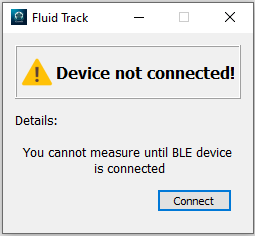
\includegraphics[width=0.4\textwidth]{Figures/ble_not_connected.png} 
    \caption{Obavijest da periferni uređaj nije povezan}
    \label{slk:ble_not_connected}
\end{figure}

Radi lakše kontrole BLE konekcijskog statusa na statusnu traku u gornji desni dio zaslona dodan je bluetooth simbol, 
što je prikazano na slici \ref{slk:ble_status}.  
Ovim pristupom korisniku se omogućava da u svakom trenutku korištenja aplikacije jednostavno može provjeriti status BLE konekcije. 

\begin{figure}[htb]
    \centering
    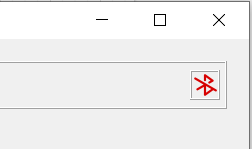
\includegraphics[width=0.4\textwidth]{Figures/cosak.png} 
    \caption{Simbol u gornjem desnom uglu koji opisuju status BLE konekcije}
    \label{slk:ble_status}
\end{figure}

\section{Postupak mjerenja}

Prvi korak pri pokretanju mjerenja je odabir između dva slučaja, mjerenje za novog pacijenta ili 
mjerenje za pacijenta koji je od ranije u bazi podataka.

\begin{figure}[htb]
    \centering
    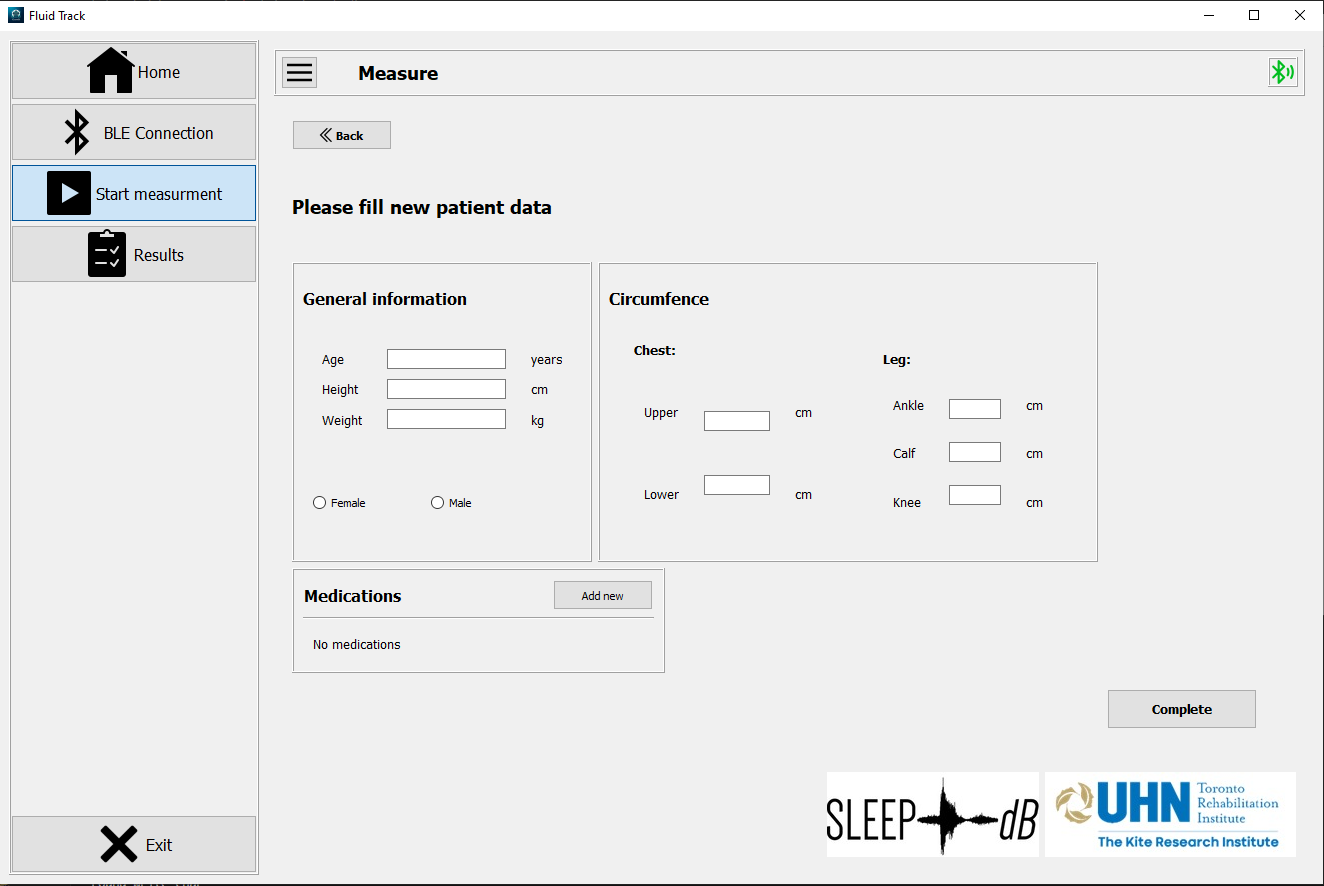
\includegraphics[width=0.85\textwidth]{Figures/patient.png} 
    \caption{Zaslon za unos podataka o pacijentu}
    \label{slk:patient}
\end{figure}

Ako se odabere novi pacijent, otvara se zaslon za unos podataka o pacijentu, prikazan na slici \ref{slk:patient}. 
Podatci koji su potrebni za daljnju analizu su dob, spol, težina, visina, obujmi prsa i noge te lijekovi koje pacijent upotrebljava. 
Nakon što korisnik popuni podatke pritiskom na tipku \texttt{Complete} pokreće se provjera ispravnosti unesenih podataka. 
Ukoliko neki od podataka nedostaju ili su u nepravilnom formatu, aplikacija obavještava korisnika skočnim prozorom s 
porukom koji točno podataka nije ispravan. 
Ako mjerenje obavljamo za pacijenta čiji su podatci od ranije u bazi podataka otvara se isti zaslon ali s popunjenim podatcima 
koje korisnik po potrebi može promijeniti.  

\begin{figure}[htb]
    \centering
    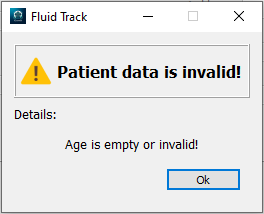
\includegraphics[width=0.4\textwidth]{Figures/invalid_data.png} 
    \caption{Primjer obavijesti neispravno unesenog podatka}
    \label{slk:invalid_data}
\end{figure}

Kada su svi podatci ispravni, otvara se prozor \ref{slk:measure} kojim se pokreče mjerenje i na kojem 
se mogu u stvarnom vremenu pratiti rezultati mjerenja. 
Mjerenje se pokreće pritiskom na tipku \texttt{Start} čime se razvijenom sustavu šalje naredba \texttt{BLE\_CMD\_START}. 
Sustav tada kontinuirano šalje podatke o izmjerenoj bioimpedanciji ispitnom okruženju. 
Ispitno okruženje iz primljenih podataka izračunava volumene tjelesnih tekućina i u stvarnom vremenu ih osvježava na grafu. 
Kako podatci pristižu, graf se automatski skalira tako da su vrijednost y osi uvijek postavljenje na ±10 \% 
od minimalne i maksimalne vrijednosti veličina prikazanih na grafu.   
Mjerenje se prekida pritiskom na tipku \texttt{Stop}.

\begin{figure}[htb]
    \centering
    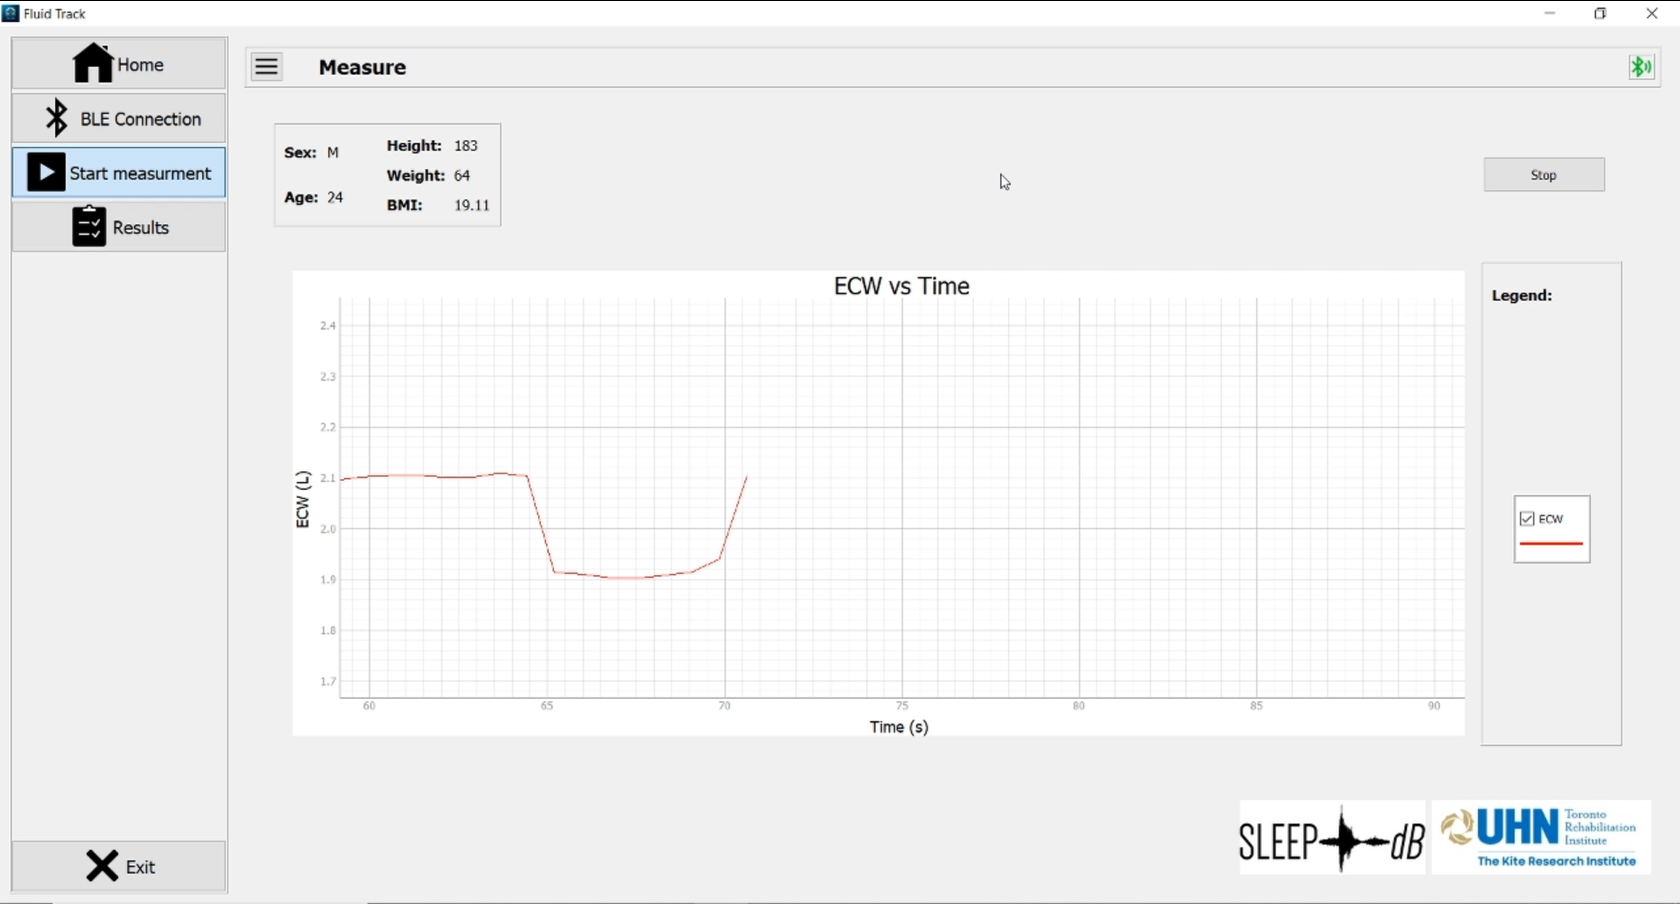
\includegraphics[width=0.85\textwidth]{Figures/measure.png} 
    \caption{Praćenje rezultata mjerenja u stvarnom vremenu}
    \label{slk:measure}
\end{figure}

Kako bi se osigurala anonimnost, pacijenti su razlikovani prema identifikacijskim brojevima, bez pohrane osobnih podataka. 
Za svakog pacijenta stvoren je folder u kojemu se nalazi csv (engl. \textit{Comma-separated values}) datoteka s njegovim 
podatcima kao i poseban folder za svako provedeno mjerenje. 
Kako bi se olakšala analiza podataka, u folderu pojedinog mjerenja podaci s pojedinih senzora spremani su u različite csv datoteke. 

\section{Prikaz rezultata}

Sustav pamti rezultate svih prijašnjih mjerenja te je u ispitno okruženje uključena podrška za prikaz prijašnjih mjerenja. 
Pritiskom na karticu izbornika \texttt{Results} otvara se skočni prozor prikazan na slici \ref{slk:select_patient} kojim korisnik odabire pacijenata 
čije rezultate mjerenje želi pogledati.

\begin{figure}[htb]
    \centering
    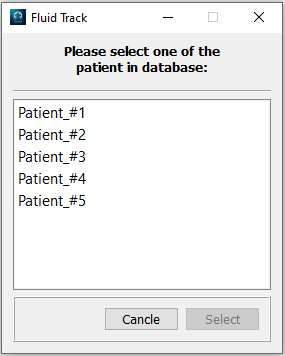
\includegraphics[width=0.3\textwidth]{Figures/select_patient.png} 
    \caption{Skočni prozor za izbor pacijenta}
    \label{slk:select_patient}
\end{figure} 

Nakon izbora pacijenta otvara se zaslon prikazan na slici \ref{slk:results_p}. 
Na zaslonu su prikazani svi ranije opisani podatci o pacijentu te popis svih njegovih mjerenja.

\begin{figure}[htb]
    \centering
    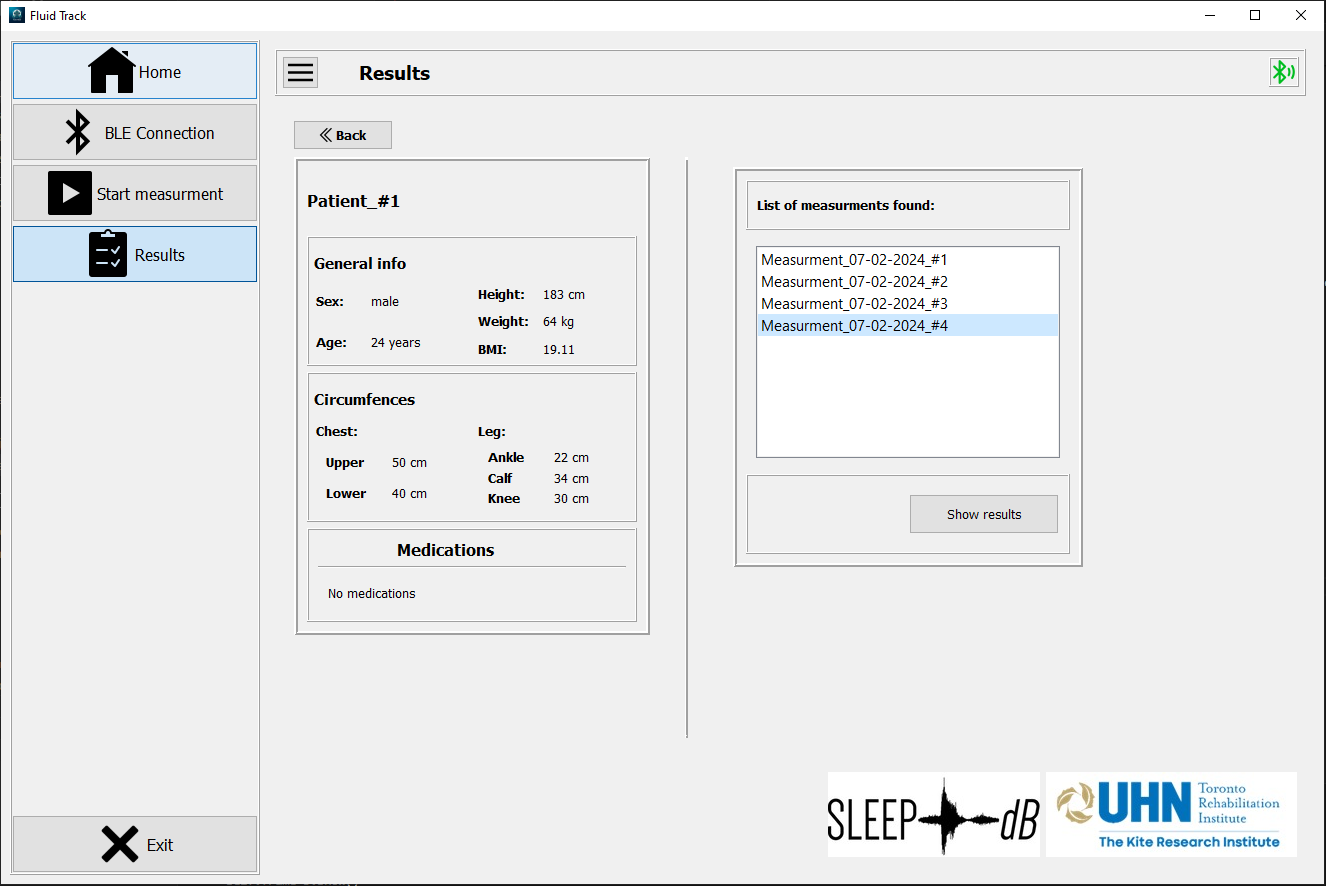
\includegraphics[width=0.85\textwidth]{Figures/results_p.png} 
    \caption{Svi podaci i provedena mjerenja za pojedinog pacijenta}
    \label{slk:results_p}
\end{figure}

klikom na konkretno mjerenje i zatim na tipku \texttt{Show results} prikazuje se zaslon koji prikazuje 
graf konkretnog mjerenja, prikazan na slici \ref{slk:results_g}. 

\begin{figure}[htb]
    \centering
    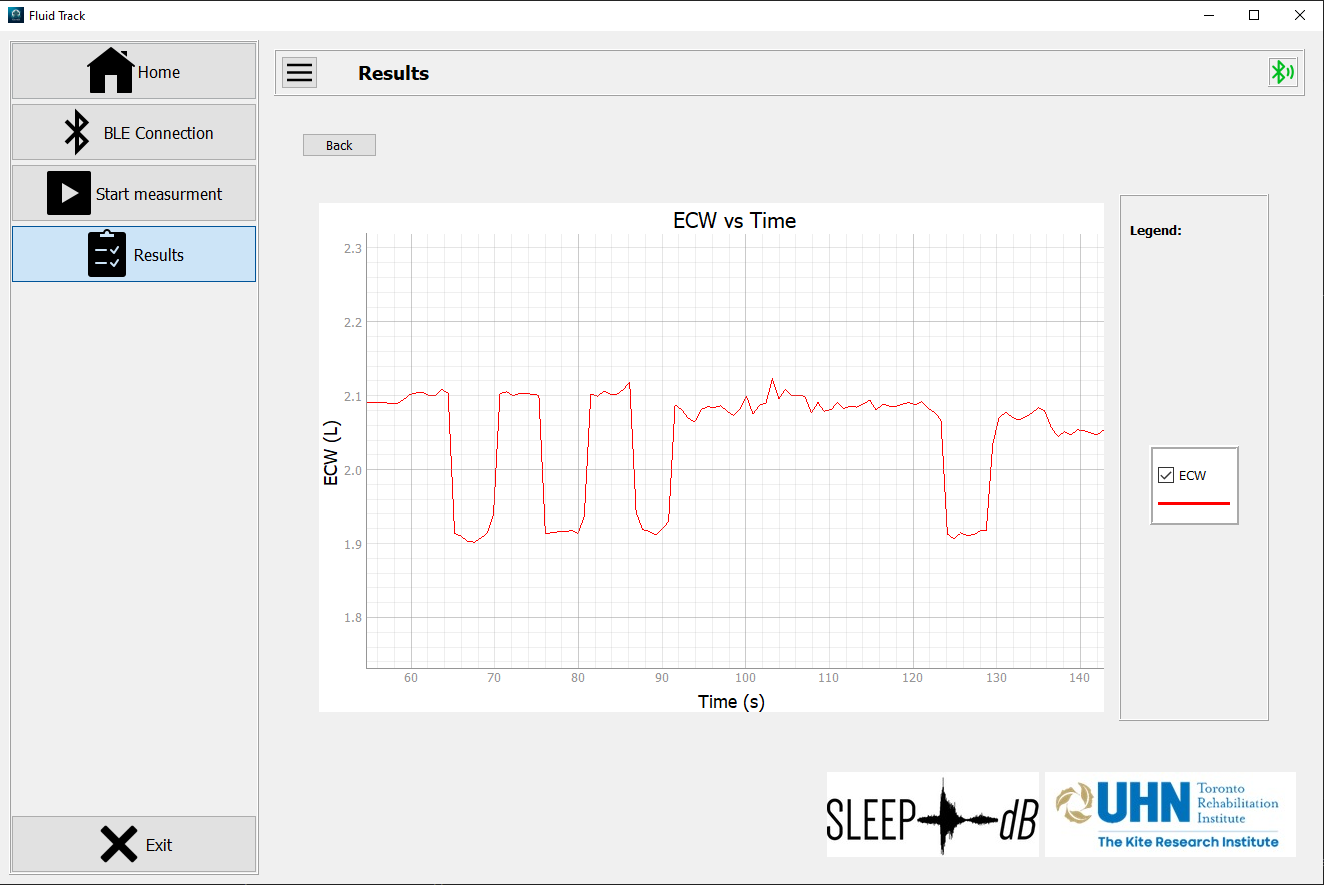
\includegraphics[width=0.85\textwidth]{Figures/results_g.png} 
    \caption{Prikaz rezultata odabranog mjerenja}
    \label{slk:results_g}
\end{figure}

\end{document}